% Chapter 4: Results and Analysis (the paper plan's "Experiments" and "Results and Discussion").
% Every number here comes from a script in the repository. Source of the preliminary
% results: scripts/01_first_garch.py, outputs in reports/first_garch/.

\section{Overview of the Chapter}
Section~\ref{sec:prelim} reports a preliminary run of the volatility models and statistical
labels on S\&P~500 data. It was run to test the pipeline and the leakage rules before any
DSE data were available, and its numbers are not the thesis results. The chapter then
states the expected outcome for each hypothesis. The main results will be added once the
experiments have been run.

\section{Preliminary Results: Volatility Models on the S\&P~500}\label{sec:prelim}

\subsection{Setup}
The data are the S\&P~500 daily closes bundled with the \texttt{arch} package, giving 5{,}030
daily log returns from 5 January 1999 to 31 December 2018. The training block (1999 to 2012)
has 3{,}520 returns and includes the 2008 crisis, validation (2013 to 2015) has 756 and test
(2016 to 2018) has 754. GARCH(1,1), EGARCH(1,1,1) and GJR(1,1,1) models with Student-$t$
innovations were fitted on the training block and run forward with frozen parameters, as
described in Chapter~\ref{ch:method}.

\subsection{Model Estimates}
Table~\ref{tab:garch-fit} gives the training-block estimates. Both asymmetric models improve
on the symmetric GARCH model by more than 120 BIC points, so negative returns raise volatility more than
positive ones in this sample. In the GJR model the symmetric coefficient $\alpha$ is
effectively zero, which means volatility responds only to negative returns. All three
models are highly persistent, and the fitted Student-$t$ degrees of freedom (8 to 10)
indicate fat tails.

\begin{table}[H]
\caption{Training-block estimates (S\&P~500, 1999 to 2012, Student-$t$ innovations).}
\label{tab:garch-fit}
\begin{center}
\small\setlength{\tabcolsep}{4pt}
\begin{tabular}{lrrrrrrr}
\hline
Model & Log-lik. & BIC & $\alpha$ & $\beta$ & $\gamma$ & Persistence & $\nu$ \\
\hline
GARCH(1,1)    & $-5230.7$ & 10502.1 & 0.081 & 0.915 & --       & 0.996 & 8.3 \\
EGARCH(1,1,1) & $-5159.7$ & 10368.5 & 0.095 & 0.986 & $-0.137$ & 0.986 & 9.5 \\
GJR(1,1,1)    & $-5165.8$ & 10380.6 & 0.000 & 0.920 & 0.142    & 0.991 & 10.4 \\
\hline
\end{tabular}
\end{center}
\small Persistence is $\alpha+\beta$ for GARCH, $\beta$ for EGARCH and $\alpha+\beta+\gamma/2$ for GJR.
\end{table}

\subsection{Residual Diagnostics}
Table~\ref{tab:garch-diag} gives p-values of the residual tests on each block. A p-value
above 0.05 means no evidence of remaining structure.

\begin{table}[H]
\caption{Residual diagnostics by block (p-values, 10 lags).}
\label{tab:garch-diag}
\begin{center}
\begin{tabular}{llrrr}
\hline
Model & Block & Ljung-Box $z$ & Ljung-Box $z^2$ & ARCH-LM \\
\hline
GARCH  & Train & 0.033 & 0.004 & 0.005 \\
       & Val   & 0.344 & 0.004 & 0.009 \\
       & Test  & 0.593 & 0.120 & 0.129 \\
EGARCH & Train & 0.015 & 0.001 & 0.001 \\
       & Val   & 0.337 & 0.231 & 0.210 \\
       & Test  & 0.250 & $<10^{-9}$ & $<10^{-6}$ \\
GJR    & Train & 0.063 & 0.008 & 0.008 \\
       & Val   & 0.361 & 0.498 & 0.419 \\
       & Test  & 0.582 & 0.354 & 0.374 \\
\hline
\end{tabular}
\end{center}
\end{table}

On the training block all three models leave some volatility clustering in the residuals
(p $< 0.01$ for $z^2$ and ARCH-LM). This is common in a sample that includes 2008, and a
richer specification may remove it. The more important result is out of sample. EGARCH, the
model with the lowest training BIC, fails badly on the test block: its squared residuals are
strongly autocorrelated (p $< 10^{-9}$). GJR passes on both validation and test, and plain
GARCH fails on validation. Selecting the volatility model by training BIC alone would have
chosen the model that generalises worst, which is why model selection in this thesis uses
validation diagnostics. The Jarque-Bera test rejects normality of the residuals for every
model and block, which supports the Student-$t$ assumption.

\subsection{Statistical Labels}
The labelling rule of Chapter~\ref{ch:method} with $p = 0.002$ was applied to the EGARCH
residuals, the model chosen by training BIC in this run, giving a cutoff of $|z_t| > 3.75$.
The naive rule on raw returns used the normal cutoff $|z| > 3.09$ for the same tail
probability. Over 5{,}030 days a correctly specified model would flag about ten.
Figure~\ref{fig:first-garch} shows the returns, the conditional volatility and the flagged
days.

\begin{figure}[H]
\centering
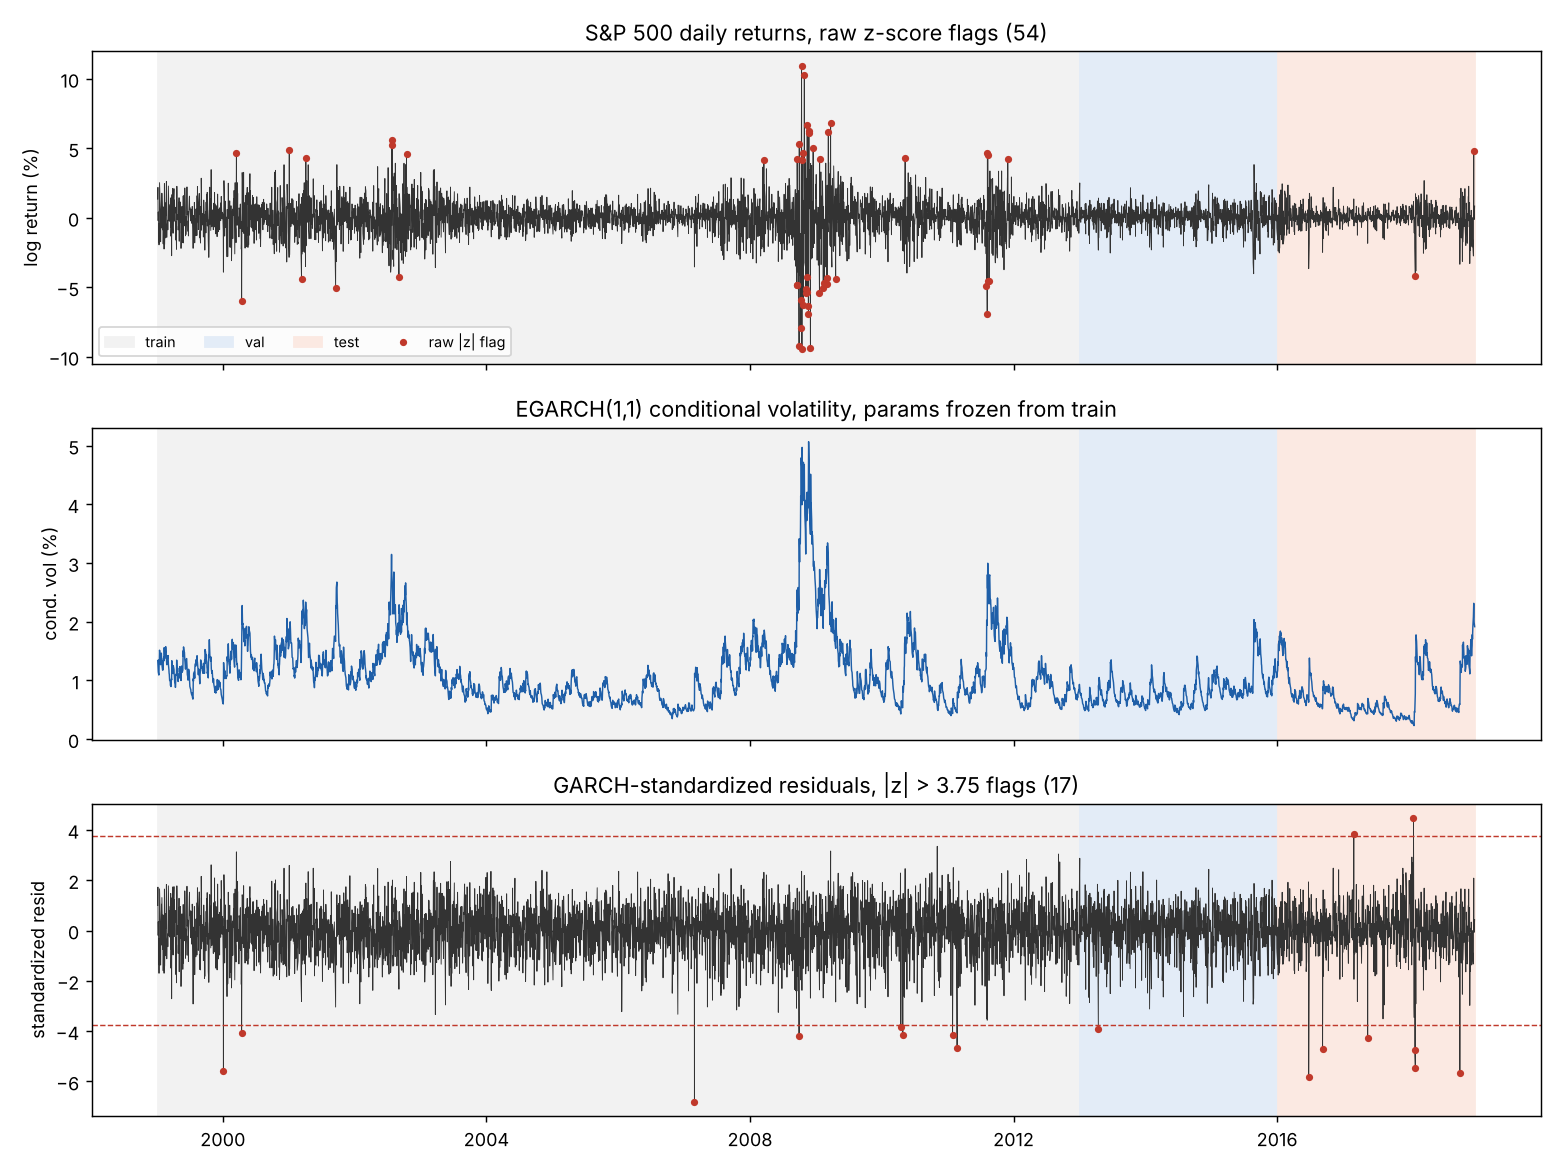
\includegraphics[width=\textwidth]{chapter4/figures/first_garch.png}
\caption{S\&P~500 daily returns with raw z-score flags (top), EGARCH conditional volatility
with parameters frozen from the training block (middle), and GARCH-standardized residuals
with flags beyond $|z|>3.75$ (bottom). Shading marks the training, validation and test
blocks.}
\label{fig:first-garch}
\end{figure}

The raw rule flagged 54 days, and 41 of them (76\%) fall in its three busiest years: 25 in
2008, 9 in 2009 and 7 in 2011. The rule mostly marks high-volatility periods rather than
individual days. The GARCH rule flagged 17 days, and its three busiest years hold 8 of them
(47\%). Its largest flags include 27 February 2007 (a global sell-off that began in
Shanghai), 29 September 2008 (the day the US House rejected the first bank rescue bill),
24 June 2016 (the day after the UK's Brexit referendum) and 5 February 2018 (a sharp rise in
US equity volatility). Of these four, the raw rule flags only the 2008 and 2018 days; the
2007 and 2016 moves were large for their own calm periods but not large compared with 2008.

One result shows a limit of the frozen-parameter setup. Eight of the 17 GARCH flags fall
in the 754 test days, where about 1.5 would be expected. In 2017 the filtered volatility
fell below anything seen in the training period (Figure~\ref{fig:first-garch}, middle
panel), so moderate moves in 2017 and early 2018 produced large standardized residuals. The
parameters, fixed at the end of 2012, do not adapt to this calmer regime. This is the
leakage-safe design behaving as intended, but it means the volatility model must be re-estimated on a rolling or expanding
window before statistical labels are fixed.

\subsection{Implications for the Main Experiments}
The preliminary run supports three decisions. The volatility model is chosen on validation
diagnostics, with GJR as the first candidate for the DSE. Statistical labels need periodic
re-estimation of the volatility model. Volatility standardization changes which days are
flagged, moving flags away from crisis periods towards days that were unusual for their own
period, which is the effect the autoencoder comparison will test. All three need to be
checked on DSE data.

\section{Expected Outcomes}
The main experiments have not been run. This section states what each hypothesis predicts
and what result would count against it, so that the results can be judged against
expectations fixed in advance.

\textbf{H1 (GARCH standardization).} The preliminary run shows that a threshold on raw
returns concentrates its flags in crisis years, while a threshold on standardized residuals
spreads them across the sample. If H1 holds, the raw-input autoencoder will show the same
pattern: more false alarms in the volatile regime and lower event-based F1 than the
standardized-input autoencoder. If the two autoencoders perform the same, or the raw model
does better on events labelled from market records, H1 is rejected for that label source.
A mixed outcome, in which standardization helps in some regimes and not others, is also
possible and will be reported as such.

\textbf{H2 (transfer).} If H2 holds, the zero-shot detector trained on global indices will
score above the statistical baselines on the DSE, and fine-tuning will narrow the gap to,
or exceed, the DSE-only detector. Standardized inputs are expected to transfer better than
raw ones, because removing each market's volatility level makes inputs from different
markets more comparable. If zero-shot transfer does not beat the baselines, the result will
show the limits of transfer into a frontier market with regulatory price distortions.

\textbf{H3 (point adjustment).} Given earlier findings on industrial
benchmarks~\cite{kim2022towards}, point-adjusted F1 is expected to exceed event-based F1 for
every detector, and the ranking of detectors may change between the two. A small gap would
also be informative: it would suggest that point adjustment matters less when most anomalies
last a single day.

\section{Main Results}
\todo{To be added after the experiments in Weeks 6 to 10: volatility model selection on DSE
data, baseline results, the raw versus standardized autoencoder comparison, transfer
results, the regime analysis and the evaluation gap.}

\section{Summary of the Chapter}
The preliminary run confirmed that the pipeline works end to end and led to three design
decisions: choose the volatility model on validation diagnostics, re-estimate it before
labels are fixed, and expect volatility standardization to move flags away from crisis
periods. The expected outcomes above set the criteria against which the main results will be
judged.
